\documentclass[11pt]{article}
\usepackage[T1]{fontenc}
\usepackage{graphicx}
\usepackage{amsmath}
\usepackage{amssymb}
\usepackage{fancyhdr}
\title{Środowisko Programisty}
\author{Filip Bestfal}
\begin{document}
\maketitle
\newpage
\tableofcontents
\listoffigures
\newpage
\begin{center}
\section{Rozdział 1}
\subsection{Podrozdział 1.1}
\end{center}
\begin{center}
Wzory skróconego mnożenia.
\end{center}
\begin{flushleft}
\label{1}
Wzór ogólny na wzory skróconego mnożenia wymyślił Isaac Newton, w postaci dwumianu Newtona.\footnote {Dwumian Newtona {$(x+y)^n$ = $${\sum_{i=1}^{n} }
{n \choose k} {a^{(n-k)}b^k}$$}}\\
Wzory skróconego mnożenia to reguły rachunkowe pozwalające uprościć obliczenia na liczbach, wielomianach i elementach, dla których obowiązująprawa przemienności oraz łączności dodawania i mnożenia, a także rozdzielności mnożenia względem dodawania.\\
Do wzorów skróconego mnożenia zalicza się między innymi wzór na:
\end{flushleft}
\begin{flushleft}
\begin{eqnarray}
(a+b)^2 = a^2 + 2ab + b^2\\
(a-b)^2 = a^2 - 2ab + b^2\\
a^2 - b^2 = (a-b)(a+b)
\end{eqnarray}
\end{flushleft}
\begin{center}
\subsubsection{Podrozdział 1.2}
\end{center}
\begin{center}
Adnotację do podrozdziału 1.1
\end{center}
ad 1. Wzór przedstawia kwadrat sumy.\\
ad 2. Wzór przedstawia kwadrat różnicy.\\
ad 3. Wzór przedstawia różnicę kwadratów.
\newpage
\begin{center}
\section{Rozdział 2}
\subsection{Podozdział 2.1}
\end{center}
\begin{center}
Wzory skróconego mnożenia trzeciej potęgi.
\end{center}
\begin{flushleft}
Ponadto istnieją również wzory skróconego mnożenia dla trzeciej potęgi.\\
A wyglądają one następująco :
\begin{flushleft}
\begin{eqnarray}
(a+b)^3 = a^3 + 3a^2b + 3ab^2 + b^3\\
(a-b)^3 = a^3 - 3a^2b + 3ab^2 - b^3\\
a^3 - b^3 = (a-b)(a^2+ab+b^2)\\
a^3 + b^3 = (a+b)(a^2-ab+b^2)
\end{eqnarray}
\end{flushleft}
\end{flushleft}
\begin{center}
\subsubsection{Podrozdział 2.2}
\end{center}
\begin{center}
Adnotację do podrozdziału 2.1
\end{center}
ad 4. Wzór przedstawia sześcian sumy.\\
ad 5. Wzór przedstawia sześcian różnicy.\\
ad 6. Wzór przedstawia różnicę sześcianów.\\
ad 7. Wzór przedstawia sumę sześcianów.\\
\newpage
\begin{center}
\section{Rozdział 3}
\subsection{Podrozdział 3.1}
\end{center}
\begin{center}
Obrazki przedstawiające graficznie wzory skróconego mnożenia.
\end{center}
\begin{figure}[ht]
\begin{center}
\label{2}
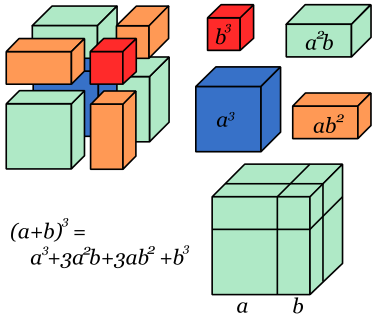
\includegraphics[width=5cm]{d.png}
\caption{Rysunek przestawiający graficznie wzór na sześcian sumy}
\label{rys_model}
\end{center}
\end{figure}
\begin{figure}[ht]
\begin{center}
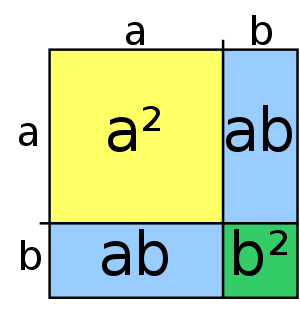
\includegraphics[width=5cm]{dd.png}
\caption{Rysunek przedstawiający graficznie kwadrat sumy}
\label{rys_model}
\end{center}
\end{figure}
\newpage
\section{Bibliografia}
\begin{thebibliography}{99}
\bibitem{pa}
\ref{1}
Pomoc ze strony : https://matematyka.net/index.php/wzory/wzory-skroconego-mnozenia
\bibitem{pa}
\ref{2}
Obrazki z arykułu wikipedii o wzorach skróconego mnożenia.
\end{thebibliography}
\end{document}